\documentclass[11pt,fleqn]{book}

\usepackage{ctex}

\usepackage[top=3cm,bottom=3cm,left=3cm,right=3cm, headsep=10pt,a4paper]{geometry} % Page margins

\usepackage{graphicx} % Required for including pictures
\graphicspath{{Pictures/}} % Specifies the directory where pictures are stored

\usepackage{tikz} % Required for drawing custom shapes
\usepackage[english]{babel} % English language/hyphenation

\usepackage{enumitem} % Customize lists
\setlist{nolistsep} % Reduce spacing between bullet points and numbered lists

\usepackage{booktabs} % Required for nicer horizontal rules in tables

\usepackage{xcolor} % Required for specifying colors by name
\definecolor{ocre}{RGB}{243,102,25} % Define the orange color used for highlighting throughout the book

\usepackage{avant} % Use the Avantgarde font for headings
%\usepackage{times} % Use the Times font for headings
\usepackage{mathptmx} % Use the Adobe Times Roman as the default text font together with math symbols from the Sym­bol, Chancery and Com­puter Modern fonts

\usepackage{microtype} % Slightly tweak font spacing for aesthetics
\usepackage[utf8]{inputenc} % Required for including letters with accents
\usepackage[T1]{fontenc} % Use 8-bit encoding that has 256 glyphs

\usepackage[style=alphabetic,citestyle=numeric,
			sorting=nyt,sortcites=true,autopunct=true,
			babel=hyphen,hyperref=true,abbreviate=false,
			backref=true,backend=biber]{biblatex}
\addbibresource{bibliography.bib} % BibTeX bibliography file
\defbibheading{bibempty}{}

\usepackage{calc} % 简单的计算功能
\usepackage{makeidx} % 创建索引
\makeindex % Tells LaTeX to create the files required for indexing

\usepackage{titletoc} % 目录操作

\contentsmargin{0cm} % Removes the default margin

% Part text styling
\titlecontents{part}[0cm]{\addvspace{20pt}\centering\large\sffamily}{}{}{}

% Chapter text styling
\titlecontents{chapter}[1.25cm] % Indentation
{\addvspace{12pt}\large\sffamily\bfseries} % Spacing and font options for chapters
{\color{ocre!60}\contentslabel[\Large\thecontentslabel]{1.25cm}\color{ocre}} % Chapter number
{\color{ocre}}  
{\color{ocre!60}\normalsize\;\titlerule*[.5pc]{.}\;\thecontentspage} % Page number

% Section text styling
\titlecontents{section}[1.25cm] % Indentation
{\addvspace{3pt}\sffamily\bfseries} % Spacing and font options for sections
{\contentslabel[\thecontentslabel]{1.25cm}} % Section number
{}
{\hfill\color{black}\thecontentspage} % Page number
[]

% Subsection text styling
\titlecontents{subsection}[1.25cm] % Indentation
{\addvspace{1pt}\sffamily\small} % Spacing and font options for subsections
{\contentslabel[\thecontentslabel]{1.25cm}} % Subsection number
{}
{\ \titlerule*[.5pc]{.}\;\thecontentspage} % Page number
[]

% List of figures
\titlecontents{figure}[0em]
{\addvspace{-5pt}\sffamily}
{\thecontentslabel\hspace*{1em}}
{}
{\ \titlerule*[.5pc]{.}\;\thecontentspage}
[]

% List of tables
\titlecontents{table}[0em]
{\addvspace{-5pt}\sffamily}
{\thecontentslabel\hspace*{1em}}
{}
{\ \titlerule*[.5pc]{.}\;\thecontentspage}
[]

%----------------------------------------------------------------------------------------
%	MINI TABLE OF CONTENTS IN PART HEADS
%----------------------------------------------------------------------------------------

% Chapter text styling
\titlecontents{lchapter}[0em] % Indenting
{\addvspace{15pt}\large\sffamily\bfseries} % Spacing and font options for chapters
{\color{ocre}\contentslabel[\Large\thecontentslabel]{1.25cm}\color{ocre}} % Chapter number
{}  
{\color{ocre}\normalsize\sffamily\bfseries\;\titlerule*[.5pc]{.}\;\thecontentspage} % Page number

% Section text styling
\titlecontents{lsection}[0em] % Indenting
{\sffamily\small} % Spacing and font options for sections
{\contentslabel[\thecontentslabel]{1.25cm}} % Section number
{}
{}

% Subsection text styling
\titlecontents{lsubsection}[.5em] % Indentation
{\normalfont\footnotesize\sffamily} % Font settings
{}
{}
{}

%----------------------------------------------------------------------------------------
%	PAGE HEADERS
%----------------------------------------------------------------------------------------

\usepackage{fancyhdr} % Required for header and footer configuration

\pagestyle{fancy}
\renewcommand{\chaptermark}[1]{\markboth{\sffamily\normalsize\bfseries\chaptername\ \thechapter.\ #1}{}} % Chapter text font settings
\renewcommand{\sectionmark}[1]{\markright{\sffamily\normalsize\thesection\hspace{5pt}#1}{}} % Section text font settings
\fancyhf{} \fancyhead[LE,RO]{\sffamily\normalsize\thepage} % Font setting for the page number in the header
\fancyhead[LO]{\rightmark} % Print the nearest section name on the left side of odd pages
\fancyhead[RE]{\leftmark} % Print the current chapter name on the right side of even pages
\renewcommand{\headrulewidth}{0.5pt} % Width of the rule under the header
\addtolength{\headheight}{2.5pt} % Increase the spacing around the header slightly
\renewcommand{\footrulewidth}{0pt} % Removes the rule in the footer
\fancypagestyle{plain}{\fancyhead{}\renewcommand{\headrulewidth}{0pt}} % Style for when a plain pagestyle is specified

% Removes the header from odd empty pages at the end of chapters
\makeatletter
\renewcommand{\cleardoublepage}{
	\clearpage\ifodd\c@page\else
	\hbox{}
	\vspace*{\fill}
	\thispagestyle{empty}
	\newpage
	\fi}

%----------------------------------------------------------------------------------------
%	THEOREM STYLES
%----------------------------------------------------------------------------------------

\usepackage{amsmath,amsfonts,amssymb,amsthm} % For math equations, theorems, symbols, etc

\newcommand{\intoo}[2]{\mathopen{]}#1\,;#2\mathclose{[}}
\newcommand{\ud}{\mathop{\mathrm{{}d}}\mathopen{}}
\newcommand{\intff}[2]{\mathopen{[}#1\,;#2\mathclose{]}}
\newtheorem{notation}{Notation}[chapter]

% Boxed/framed environments
\newtheoremstyle{ocrenumbox}% % Theorem style name
{0pt}% Space above
{0pt}% Space below
{\normalfont}% % Body font
{}% Indent amount
{\small\bf\sffamily\color{ocre}}% % Theorem head font
{\;}% Punctuation after theorem head
{0.25em}% Space after theorem head
{\small\sffamily\color{ocre}\thmname{#1}\nobreakspace\thmnumber{\@ifnotempty{#1}{}\@upn{#2}}% Theorem text (e.g. Theorem 2.1)
	\thmnote{\nobreakspace\the\thm@notefont\sffamily\bfseries\color{black}---\nobreakspace#3.}} % Optional theorem note
\renewcommand{\qedsymbol}{$\blacksquare$}% Optional qed square

\newtheoremstyle{blacknumex}% Theorem style name
{5pt}% Space above
{5pt}% Space below
{\normalfont}% Body font
{} % Indent amount
{\small\bf\sffamily}% Theorem head font
{\;}% Punctuation after theorem head
{0.25em}% Space after theorem head
{\small\sffamily{\tiny\ensuremath{\blacksquare}}\nobreakspace\thmname{#1}\nobreakspace\thmnumber{\@ifnotempty{#1}{}\@upn{#2}}% Theorem text (e.g. Theorem 2.1)
	\thmnote{\nobreakspace\the\thm@notefont\sffamily\bfseries---\nobreakspace#3.}}% Optional theorem note

\newtheoremstyle{blacknumbox} % Theorem style name
{0pt}% Space above
{0pt}% Space below
{\normalfont}% Body font
{}% Indent amount
{\small\bf\sffamily}% Theorem head font
{\;}% Punctuation after theorem head
{0.25em}% Space after theorem head
{\small\sffamily\thmname{#1}\nobreakspace\thmnumber{\@ifnotempty{#1}{}\@upn{#2}}% Theorem text (e.g. Theorem 2.1)
	\thmnote{\nobreakspace\the\thm@notefont\sffamily\bfseries---\nobreakspace#3.}}% Optional theorem note

% Non-boxed/non-framed environments
\newtheoremstyle{ocrenum}% % Theorem style name
{5pt}% Space above
{5pt}% Space below
{\normalfont}% % Body font
{}% Indent amount
{\small\bf\sffamily\color{ocre}}% % Theorem head font
{\;}% Punctuation after theorem head
{0.25em}% Space after theorem head
{\small\sffamily\color{ocre}\thmname{#1}\nobreakspace\thmnumber{\@ifnotempty{#1}{}\@upn{#2}}% Theorem text (e.g. Theorem 2.1)
	\thmnote{\nobreakspace\the\thm@notefont\sffamily\bfseries\color{black}---\nobreakspace#3.}} % Optional theorem note
\renewcommand{\qedsymbol}{$\blacksquare$}% Optional qed square
\makeatother

% Defines the theorem text style for each type of theorem to one of the three styles above
\newcounter{dummy} 
\numberwithin{dummy}{section}
\theoremstyle{ocrenumbox}
\newtheorem{theoremeT}[dummy]{Theorem}
\newtheorem{problem}{Problem}[chapter]
\newtheorem{exerciseT}{Exercise}[chapter]
\theoremstyle{blacknumex}
\newtheorem{exampleT}{Example}[chapter]
\theoremstyle{blacknumbox}
\newtheorem{vocabulary}{Vocabulary}[chapter]
\newtheorem{definitionT}{Definition}[section]
\newtheorem{corollaryT}[dummy]{Corollary}
\theoremstyle{ocrenum}
\newtheorem{proposition}[dummy]{Proposition}

%----------------------------------------------------------------------------------------
%	DEFINITION OF COLORED BOXES
%----------------------------------------------------------------------------------------

\RequirePackage[framemethod=default]{mdframed} % Required for creating the theorem, definition, exercise and corollary boxes

% Theorem box
\newmdenv[skipabove=7pt,
skipbelow=7pt,
backgroundcolor=black!5,
linecolor=ocre,
innerleftmargin=5pt,
innerrightmargin=5pt,
innertopmargin=5pt,
leftmargin=0cm,
rightmargin=0cm,
innerbottommargin=5pt]{tBox}

% Exercise box	  
\newmdenv[skipabove=7pt,
skipbelow=7pt,
rightline=false,
leftline=true,
topline=false,
bottomline=false,
backgroundcolor=ocre!10,
linecolor=ocre,
innerleftmargin=5pt,
innerrightmargin=5pt,
innertopmargin=5pt,
innerbottommargin=5pt,
leftmargin=0cm,
rightmargin=0cm,
linewidth=4pt]{eBox}	

% Definition box
\newmdenv[skipabove=7pt,
skipbelow=7pt,
rightline=false,
leftline=true,
topline=false,
bottomline=false,
linecolor=ocre,
innerleftmargin=5pt,
innerrightmargin=5pt,
innertopmargin=0pt,
leftmargin=0cm,
rightmargin=0cm,
linewidth=4pt,
innerbottommargin=0pt]{dBox}	

% Corollary box
\newmdenv[skipabove=7pt,
skipbelow=7pt,
rightline=false,
leftline=true,
topline=false,
bottomline=false,
linecolor=gray,
backgroundcolor=black!5,
innerleftmargin=5pt,
innerrightmargin=5pt,
innertopmargin=5pt,
leftmargin=0cm,
rightmargin=0cm,
linewidth=4pt,
innerbottommargin=5pt]{cBox}

% Creates an environment for each type of theorem and assigns it a theorem text style from the "Theorem Styles" section above and a colored box from above
\newenvironment{theorem}{\begin{tBox}\begin{theoremeT}}{\end{theoremeT}\end{tBox}}
\newenvironment{exercise}{\begin{eBox}\begin{exerciseT}}{\hfill{\color{ocre}\tiny\ensuremath{\blacksquare}}\end{exerciseT}\end{eBox}}				  
\newenvironment{definition}{\begin{dBox}\begin{definitionT}}{\end{definitionT}\end{dBox}}	
\newenvironment{example}{\begin{exampleT}}{\hfill{\tiny\ensuremath{\blacksquare}}\end{exampleT}}		
\newenvironment{corollary}{\begin{cBox}\begin{corollaryT}}{\end{corollaryT}\end{cBox}}	

%----------------------------------------------------------------------------------------
%	REMARK ENVIRONMENT
%----------------------------------------------------------------------------------------

\newenvironment{remark}[1]{\par\vspace{10pt}\small % Vertical white space above the remark and smaller font size
	\begin{list}{}{
			\leftmargin=35pt % Indentation on the left
			\rightmargin=25pt}\item\ignorespaces % Indentation on the right
		\makebox[-2.5pt]{\begin{tikzpicture}[overlay]
			\node[draw=ocre!60,line width=1pt,circle,fill=ocre!25,font=\sffamily\bfseries,inner sep=2pt,outer sep=0pt] at (-15pt,0pt){\textcolor{ocre}{#1}};\end{tikzpicture}} % Orange R in a circle
		\advance\baselineskip -1pt}{\end{list}\vskip5pt} % Tighter line spacing and white space after remark

%----------------------------------------------------------------------------------------
%	SECTION NUMBERING IN THE MARGIN
%----------------------------------------------------------------------------------------

\makeatletter
\renewcommand{\@seccntformat}[1]{\llap{\textcolor{ocre}{\csname the#1\endcsname}\hspace{1em}}}                    
\renewcommand{\section}{\@startsection{section}{1}{\z@}
	{-4ex \@plus -1ex \@minus -.4ex}
	{1ex \@plus.2ex }
	{\normalfont\large\sffamily\bfseries}}
\renewcommand{\subsection}{\@startsection {subsection}{2}{\z@}
	{-3ex \@plus -0.1ex \@minus -.4ex}
	{0.5ex \@plus.2ex }
	{\normalfont\sffamily\bfseries}}
\renewcommand{\subsubsection}{\@startsection {subsubsection}{3}{\z@}
	{-2ex \@plus -0.1ex \@minus -.2ex}
	{.2ex \@plus.2ex }
	{\normalfont\small\sffamily\bfseries}}                        
\renewcommand\paragraph{\@startsection{paragraph}{4}{\z@}
	{-2ex \@plus-.2ex \@minus .2ex}
	{.1ex}
	{\normalfont\small\sffamily\bfseries}}

%----------------------------------------------------------------------------------------
%	PART HEADINGS
%----------------------------------------------------------------------------------------

% numbered part in the table of contents
\newcommand{\@mypartnumtocformat}[2]{%
	\setlength\fboxsep{0pt}%
	\noindent\colorbox{ocre!20}{\strut\parbox[c][.7cm]{\ecart}{\color{ocre!70}\Large\sffamily\bfseries\centering#1}}\hskip\esp\colorbox{ocre!40}{\strut\parbox[c][.7cm]{\linewidth-\ecart-\esp}{\Large\sffamily\centering#2}}}%
%%%%%%%%%%%%%%%%%%%%%%%%%%%%%%%%%%
% unnumbered part in the table of contents
\newcommand{\@myparttocformat}[1]{%
	\setlength\fboxsep{0pt}%
	\noindent\colorbox{ocre!40}{\strut\parbox[c][.7cm]{\linewidth}{\Large\sffamily\centering#1}}}%
%%%%%%%%%%%%%%%%%%%%%%%%%%%%%%%%%%
\newlength\esp
\setlength\esp{4pt}
\newlength\ecart
\setlength\ecart{1.2cm-\esp}
\newcommand{\thepartimage}{}%
\newcommand{\partimage}[1]{\renewcommand{\thepartimage}{#1}}%
\def\@part[#1]#2{%
	\ifnum \c@secnumdepth >-2\relax%
	\refstepcounter{part}%
	\addcontentsline{toc}{part}{\texorpdfstring{\protect\@mypartnumtocformat{\thepart}{#1}}{\partname~\thepart\ ---\ #1}}
	\else%
	\addcontentsline{toc}{part}{\texorpdfstring{\protect\@myparttocformat{#1}}{#1}}%
	\fi%
	\startcontents%
	\markboth{}{}%
	{\thispagestyle{empty}%
		\begin{tikzpicture}[remember picture,overlay]%
		\node at (current page.north west){\begin{tikzpicture}[remember picture,overlay]%	
			\fill[ocre!20](0cm,0cm) rectangle (\paperwidth,-\paperheight);
			\node[anchor=north] at (4cm,-3.25cm){\color{ocre!40}\fontsize{220}{100}\sffamily\bfseries\@Roman\c@part}; 
			\node[anchor=south east] at (\paperwidth-1cm,-\paperheight+1cm){\parbox[t][][t]{8.5cm}{
					\printcontents{l}{0}{\setcounter{tocdepth}{1}}%
			}};
			\node[anchor=north east] at (\paperwidth-1.5cm,-3.25cm){\parbox[t][][t]{15cm}{\strut\raggedleft\color{white}\fontsize{30}{30}\sffamily\bfseries#2}};
			\end{tikzpicture}};
\end{tikzpicture}}%
\@endpart}
\def\@spart#1{%
\startcontents%
\phantomsection
{\thispagestyle{empty}%
	\begin{tikzpicture}[remember picture,overlay]%
	\node at (current page.north west){\begin{tikzpicture}[remember picture,overlay]%	
		\fill[ocre!20](0cm,0cm) rectangle (\paperwidth,-\paperheight);
		\node[anchor=north east] at (\paperwidth-1.5cm,-3.25cm){\parbox[t][][t]{15cm}{\strut\raggedleft\color{white}\fontsize{30}{30}\sffamily\bfseries#1}};
		\end{tikzpicture}};
\end{tikzpicture}}
\addcontentsline{toc}{part}{\texorpdfstring{%
	\setlength\fboxsep{0pt}%
	\noindent\protect\colorbox{ocre!40}{\strut\protect\parbox[c][.7cm]{\linewidth}{\Large\sffamily\protect\centering #1\quad\mbox{}}}}{#1}}%
\@endpart}
\def\@endpart{\vfil\newpage
\if@twoside
\if@openright
\null
\thispagestyle{empty}%
\newpage
\fi
\fi
\if@tempswa
\twocolumn
\fi}

%----------------------------------------------------------------------------------------
%	CHAPTER HEADINGS
%----------------------------------------------------------------------------------------

% A switch to conditionally include a picture, implemented by  Christian Hupfer
\newif\ifusechapterimage
\usechapterimagetrue
\newcommand{\thechapterimage}{}%
\newcommand{\chapterimage}[1]{\ifusechapterimage\renewcommand{\thechapterimage}{#1}\fi}%
\def\@makechapterhead#1{%
{\parindent \z@ \raggedright \normalfont
\ifnum \c@secnumdepth >\m@ne
\if@mainmatter
\begin{tikzpicture}[remember picture,overlay]
\node at (current page.north west)
{\begin{tikzpicture}[remember picture,overlay]
	\node[anchor=north west,inner sep=0pt] at (0,0) {\ifusechapterimage\includegraphics[width=\paperwidth]{\thechapterimage}\fi};
	\draw[anchor=west] (\Gm@lmargin,-9cm) node [line width=2pt,rounded corners=15pt,draw=ocre,fill=white,fill opacity=0.5,inner sep=15pt]{\strut\makebox[22cm]{}};
	\draw[anchor=west] (\Gm@lmargin+.3cm,-9cm) node {\huge\sffamily\bfseries\color{black}\thechapter. #1\strut};
	\end{tikzpicture}};
\end{tikzpicture}
\else
\begin{tikzpicture}[remember picture,overlay]
\node at (current page.north west)
{\begin{tikzpicture}[remember picture,overlay]
\node[anchor=north west,inner sep=0pt] at (0,0) {\ifusechapterimage\includegraphics[width=\paperwidth]{\thechapterimage}\fi};
\draw[anchor=west] (\Gm@lmargin,-9cm) node [line width=2pt,rounded corners=15pt,draw=ocre,fill=white,fill opacity=0.5,inner sep=15pt]{\strut\makebox[22cm]{}};
\draw[anchor=west] (\Gm@lmargin+.3cm,-9cm) node {\huge\sffamily\bfseries\color{black}#1\strut};
\end{tikzpicture}};
\end{tikzpicture}
\fi\fi\par\vspace*{270\p@}}}

%-------------------------------------------

\def\@makeschapterhead#1{%
\begin{tikzpicture}[remember picture,overlay]
\node at (current page.north west)
{\begin{tikzpicture}[remember picture,overlay]
\node[anchor=north west,inner sep=0pt] at (0,0) {\ifusechapterimage\includegraphics[width=\paperwidth]{\thechapterimage}\fi};
\draw[anchor=west] (\Gm@lmargin,-9cm) node [line width=2pt,rounded corners=15pt,draw=ocre,fill=white,fill opacity=0.5,inner sep=15pt]{\strut\makebox[22cm]{}};
\draw[anchor=west] (\Gm@lmargin+.3cm,-9cm) node {\huge\sffamily\bfseries\color{black}#1\strut};
\end{tikzpicture}};
\end{tikzpicture}
\par\vspace*{270\p@}}
\makeatother

%----------------------------------------------------------------------------------------
%	HYPERLINKS IN THE DOCUMENTS
%----------------------------------------------------------------------------------------

\usepackage{hyperref}
\hypersetup{hidelinks,backref=true,pagebackref=true,hyperindex=true,colorlinks=false,breaklinks=true,urlcolor= ocre,bookmarks=true,bookmarksopen=false,pdftitle={Title},pdfauthor={Author}}
\usepackage{bookmark}
\bookmarksetup{
open,
numbered,
addtohook={%
\ifnum\bookmarkget{level}=0 % chapter
\bookmarksetup{bold}%
\fi
\ifnum\bookmarkget{level}=-1 % part
\bookmarksetup{color=ocre,bold}%
\fi
}
}

\begin{document}

\begingroup
\thispagestyle{empty}
\begin{tikzpicture}[remember picture,overlay]
\coordinate [below=12cm] (midpoint) at (current page.north);
\node at (current page.north west)
{\begin{tikzpicture}[remember picture,overlay]
\node[anchor=north west,inner sep=0pt] at (0,0) {
\includegraphics[width=\paperwidth]{background}}; % Background image
\draw[anchor=north] (midpoint) node [fill=ocre!30!white,fill opacity=0.6,text opacity=1,inner sep=1cm]{\Huge\centering\bfseries\sffamily\parbox[c][][t]{\paperwidth}{\centering 2017年秋超越学科认知基础\\[15pt] % Book title
{\Large 课程学习报告}\\[20pt] % Subtitle
{\huge 本课程全体同学}}}; % Author name
\end{tikzpicture}};
\end{tikzpicture}
\vfill
\endgroup

%----------------------------------------------------------------------------------------
%	COPYRIGHT PAGE
%----------------------------------------------------------------------------------------

\newpage
~\vfill
\begin{figure}[h]
	\centering
\includegraphics[width=5cm]{123.jpg}
\end{figure}


\begin{center}
	{\sffamily
		\textbf{\copyright 2017 \href{http://toyhouse.cc/wiki/index.php/Seven_Brief_Lessons_on_Physics}{\textbf{超越学科界限的认知基础}}}\\
		\textsc{Creative Commons}\\
		
		署名-相同方式共享 3.0 未本地化版本\\
		\href{https://creativecommons.org/licenses/by-sa/3.0/legalcode}{(CC BY-SA 3.0)}\\[12pt]
		
\includegraphics{Pictures/license.png}\\[12pt]
	}
\end{center}


%----------------------------------------------------------------------------------------
%	TABLE OF CONTENTS
%----------------------------------------------------------------------------------------

%\usechapterimagefalse % If you don't want to include a chapter image, use this to toggle images off - it can be enabled later with \usechapterimagetrue

\chapterimage{chapter_head_1.pdf} % Table of contents heading image

\pagestyle{empty} % No headers

\tableofcontents % Print the table of contents itself

\cleardoublepage % Forces the first chapter to start on an odd page so it's on the right

\pagestyle{fancy} % Print headers again

%----------------------------------------------------------------------------------------
%	PART
%----------------------------------------------------------------------------------------

%\part{课程简介}

%----------------------------------------------------------------------------------------
%	CHAPTER 1
%----------------------------------------------------------------------------------------

\chapterimage{chapter_head_2.pdf} % Chapter heading image

\chapter{课程主题}

\section{English version of introduction}

This course is developed with Xinya Residential Colledge in mind. Students of this course are expected to come from many different disciplinary backgrounds, i.e. Theoretical Mechanics, Law school, Architecture, and Life Sciences. The goal is to use Cognitive Foundation as a common framework to help students find a way to intellectually communicate with students from other disciplinary-domains. To ensure deeper engagement on the intellectual level, we will mobilize students to use a Digital Publishing Workflow to share weekly learning summary and co-author a report on topics of their collective interests. The topics chosen in this course will be directed toward some of the most foundational phenomonen that relates to human cognitive behavior, both individually and groupwise. Key concepts in modern science such as Non-Local Phenomenon in Quantum Physics, Distributed vs. Centralized Communication processes in IT systems, Distributive Justice in Legal systems, and Design Thinking activities in Architecture Decision, and Interconnectivity in Life Sciences.

\section{中文简介}
本课程是由新雅书院建议开发。这是第一次以四个不同学院、分属不同学科的同学为参与对象的一门课程,初期以来自钱学森力学班、法学院、建筑学院和生命学院的本科生为主。因此,本课程将以跨学科的认知基础为主题,让不同学科背景的同学能从各自的基础认知架构出发,帮助其他学科的同学,共同凝聚一个可以从不同视角相互支撑或相互挑战的学习内容。 教学过程中,同学和老师将共同参与完成分布式数字出版工作流,从而使同学能体验到群体合作开发及累积知识的现代求学方式。建立在基础的知识体系之上,同学与老师的共同讨论将不断增添及修正课堂内容,从而让这门课程能够不断地自我完善。

本课程将涉及以下几个相关学科的内容:量子非定域(Non-Local)的物理现象、互联网技术的分布式架构、法学理论中的分布式公正性(Distributive Justice)、生命科学和建筑学院的设计思维。

\section{逻辑模型}

当代,由于科学工程等学科任务的复杂度不断上升,依靠传统的方法与手段已经很难以组织起一个有力的解决问题的框架。逻辑模型的提出与推动正是为了顺应缓解这种需要。本门课程十分注意逻辑模型的使用,无论是课程学生每一次的个人报告还是小组的团队报告,都带有本次任务的逻辑模型。通过逻辑模型的训练,学生们的思维严谨性与可塑性都得到了很好的加强。

这里为了能够更好地介绍逻辑模型,采用了Wikipedia上面关于Logic Model的定义。或许定义还算不上严谨准确,但是我们认为对于理解逻辑模型的本质,了解逻辑模型的作用来说,已经是足够的。

图1.1是我们这门课的逻辑模型,在我们的实践过程中与模型有一定的偏差,作出了一定的修正。如图1.2所示:

\begin{figure}[h]
	\centering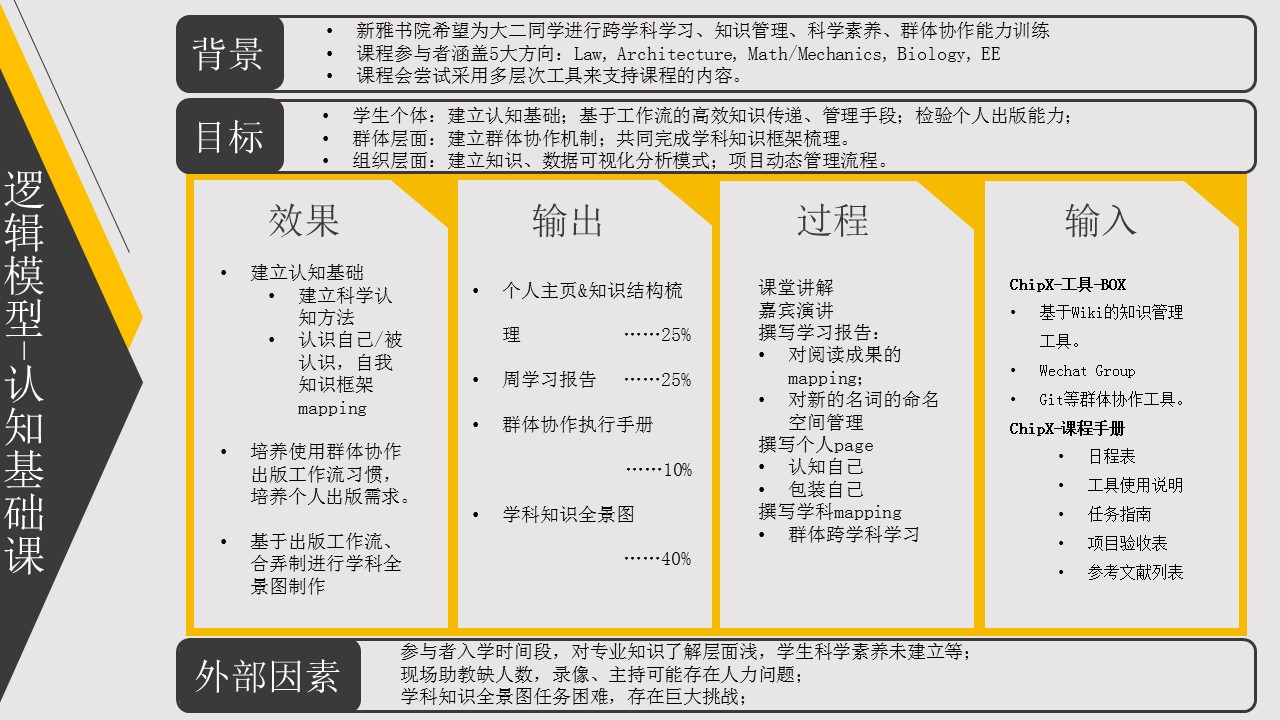
\includegraphics[width=15cm]{1.jpg}
	\caption{本门课程初始逻辑模型}
\end{figure}

\begin{figure}[h]
	\centering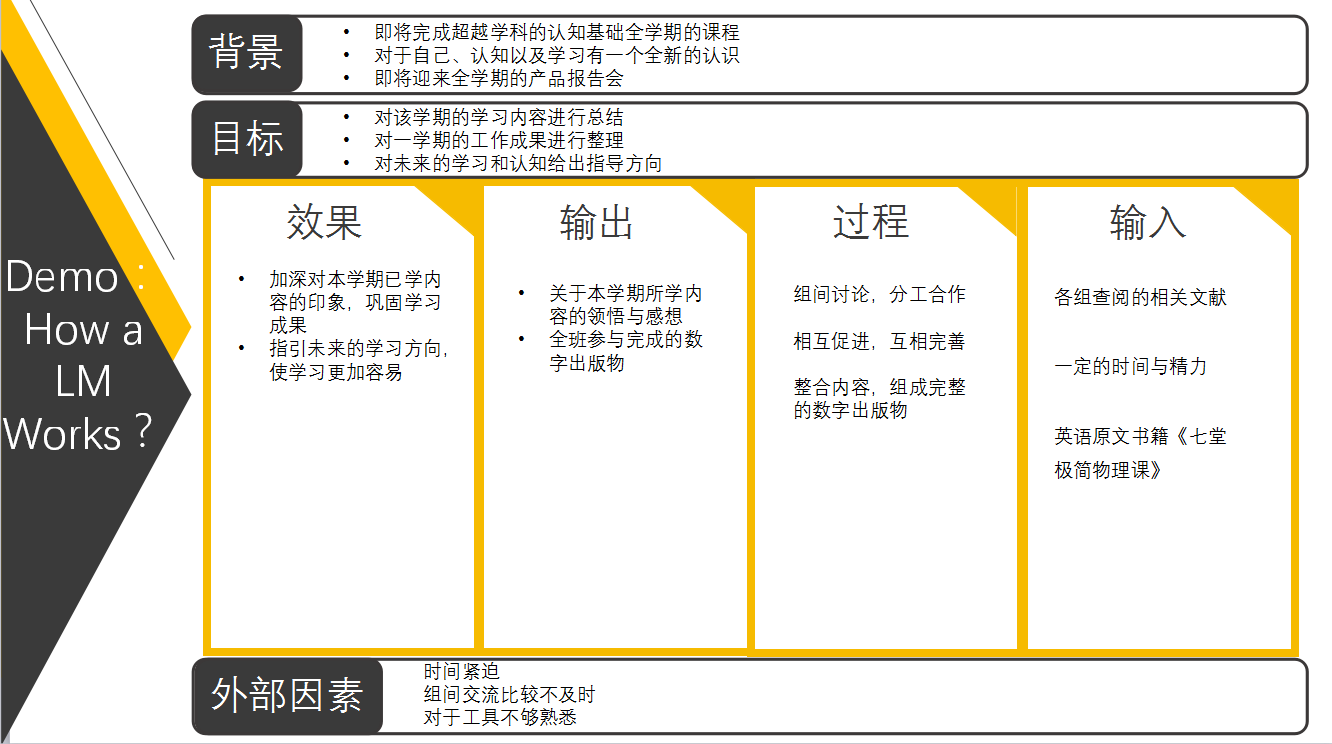
\includegraphics[width=15cm]{12.png}
	\caption{本门课程迭代后的逻辑模型}
\end{figure}

\chapter{成果与收获}

\section{期末成果}

在本门课程的学习中,我们每一名学生都学习到了许多事物,同时对于认知科学的部分知识增进了自己的了解。主要实体成果就是《七堂极简物理课》的翻译。我们一致认为,这本书深入浅出,讲解清晰透彻,既满足了物理学“门外汉”的学习需要,同时也在一定程度上概括了物理学家们认识世界的基本过程,对于我们深入理解认知有着很大的帮助。

通过这本书的翻译,我们希望收获到的不仅仅是一本译著,更多的是对于认识过程的深入理解。当然,如果能够借由这一本书的翻译与世界各地的优秀学生交流分享体会的话,那也是更好的。

\section{各小组成员的学习心得与体会}

\subsection{第一组}

\begin{remark}{费}
	这一学期在种种机缘巧合之下,我选择了《超越学科的认知基础》这门课。从学期初老师所讲的认知、隐喻与函数,再到后来的空间隐喻、本体隐喻与系统隐喻,再到深奥难懂的范畴论及其中的函数、函子与自然转换,尽管从知识层面上,我还没有达到融会贯通的境地,但是至少,我初步了解了认知的基本过程与基本方法。如果非要我说学习这些的目的,我觉得这些知识是我们认知世界的桥梁——就像牛顿定律是我们认识经典力学框架下世界的基础一眼,只不过由于认识与学习之间的关系的复杂性,理清认识的过程就能在很大程度上帮助我们理解世界,在这个人工智能越来越热的大背景下,如果仅仅靠记忆知识,我们永远无法超过现在的计算机,但是在强人工智能出现之前,如果我们能深刻地把握认知的基本规律,一方面我们能为自己创造存在的价值,另一方面我们也能为人工智能搭建其一种理论上的框架:如果我们能够深入理解人认知世界的方式,那么我们又何尝不能将这一方式应用于未来人工智能的开发与应用中呢?所以说,尽管临近学期尾声,但是这门课所给予我的影响,给予我的思考,是不会走进尾声的。同时我也要感谢老师和助教在我们学习的过程中为我们提供了一个很好的学习平台,无论是Wiki、Git、Phabricator、Modelica、Mathematica都是很好的帮助我们认识世界的工具,我也希望着,这些工具能够在我未来的学习生活中发挥越来越大的作用。对于各种软件的使用,我也有着自己的感受与想法。Wiki:作为一个并没有紧跟互联网时代潮流的人,在老师最开始讲Wiki时,我脑海中除了Wikipedia和Wikimedia Commons之外没有出现过其它东西。经过一学期的学习和使用,我越来越能感受到Wiki的好处与意义,在我看来主要表现为以下几点:1.易于编辑和更改:Wiki相当于在网上开辟了一段空间,使得我们可以在其中自在的书写自己的学习心得与学习感悟;2.历史记录:Wiki可以将每次的修改记录都进行保存,而且提供了很方便的查询比较操作接口;3.Wiki上可以进行讨论:对于自己或他人所写内容均可在讨论页面中书写自己的感受,表达自己的观点,相当于为每一个词条都设立了一个专门专用的讨论区。这学期,我每周都坚持使用Wiki记录自己的学习心得,受益良多。Git:同样地,Git这种工具我在以前闻所未闻,本学期我们所用的Git主要是Github这种工具。起初我还是难以理解这种工具的存在意义,但后来随着自己学习的深入,我渐渐发现Git这种工具实际上在许多方面都发挥着不可替代的作用。相较于Wiki,Git上可以留存的文件的种类以及数目都更多,相应地使用弹性就更大,我们可以发现有许多工具都是直接存留在Git上,既便于查看,也便于分享交流。作为Git中的一种主要实现,Github在充分保留了以上几个特点后,还使得交互界面更加和谐,更加便于我们使用。从这一角度来看,Git实在是在当今时代紧跟时代步伐进行学习的一个不可或缺的工具。Phabricator:Phabricator在许多方面与Git有相似之处,但是在细节上还有一些差异,在我看来主要差异大致如下:1.Git的主要用处在于设置一个网上交互的文件中转站,而Phabricator的主要作用是安排任务。从我们团队Project的角度来说,Phabricator在可以充分完成文件交互这一基本功能的基础上,还可以对我们的任务进行分门别类,这样可以更为有效地组织起我们的团队工作;2.Phabricator可以更好地兼容我们的想法,这一点上它又继承了Wiki的优势。Modelica:Modelica这款仿真软件在之前我基本上都没有接触过,尽管我到现在也没有使用Modelica作出什么有意义的仿真成果,但是至少在那节课上,我意识到了这款仿真软件的优秀之处。我想更多的感想还是要放到以后,等到我真正应用这款软件作出一些有趣有用的成果时才可以说明吧。Mathematica:这些软件中,或许只有Mathematica我还是比较熟悉的。从学期初的Mathematica的使用讲解,到后来自己用Mathematica解决一些实际的问题,希望自己以后能够学会不仅仅使用Mathematica进行符号计算,还能够学会其中机器学习的基本思想与使用方法。总体而言,作为与Matlab风格迥异的数学软件,或许Mathematica更容易接近于我们的认知过程,也使得我们有很大必要掌握这种软件的使用。
\end{remark}

\begin{remark}{张}
     一学期的时光犹如白驹过隙,转瞬即逝,曾经懵懂无比,带着好奇心走进李兆基大楼的我也在这一个学期的学习中得到了成长与突破。遥想第一节课听到“认知”,“隐喻”,“范畴论”等概念时的不知所措,仿佛就在昨日,第一节课听到的任务当时感觉完全无法做到,但通过我们一个班十几位同学的共同努力,居然真的完成了一本数字出版物的制作。与科技大牛,外国大学生,台湾清华大学的教授的交流都让人受益良多,待在象牙塔里的我们不了解外面的世界,顾老师就把外面的世界拉到了我们的课堂上,真的感觉非常nice。从第一节课就重点提到的逻辑模型,给了我一个重新认识问题的方法,思考问题的顺序决定了我们能达到的高度。顾老师不止一次地强调希望我们作为清华大学的学生,在这门课上能刷新对自己的标准,那么我想,至少在工具使用这方面在上这门课前我是绝对落伍了的。Wiki,Github,Phabricator,Mathematics乃至LaTeX等工具我之前几乎完全没有接触过,根本无法达到信息化时代普通大学生的基本要求。一个学期下来,Wiki已经用得得心应手,Github这个工具也成为我寻找开源资料的重要场所,Phabricator这个可以让我们随时随地讨论工作进度,最终能有所结果的工具可以说是十分赞了,有网络的地方就有我们思想碰撞的火花。

     现在,我的认知已经发生了翻天覆地的变化,我们在寻找超越学科的认知的道路上也已经迈出了重要的步伐。而大有若无,随时随地还能开花结果的学习空间也在慢慢变为现实,这门课上的内容或许很久以后回想起来依然能带给我不一样的收获。我天性愚钝,或许顾老师深邃的思想只能略窥一二,但是时间会让我知道谁才是真正的智者。感谢顾老师,周工和各位助教一学期以来的付出和努力,也谢谢一直不离不弃给我支持的队友,作为即将开放的Wiki的首批见证人,我的心里满是荣幸。
\end{remark}

\begin{remark}{黄}
	我主要负责了这几周合弄制宪章的书写和修订,总结几条规律:首先每一周的任务就像一个小的项目,它需要根据每个圈子的特点来进行相应的任务接受,任务确定,任务分配,任务推动,任务汇总,任务查收,问题修改等过程,那么如何建立一个良好的和弄制体制就显得非常的重要,我通过这几周的总结,我认为根据每个人不同的特点进行任务的分配非常的重要,因此这些周的任务分配,我们结合了所有成员的特点进行分配,英语水平高的同学主要负责翻译修改,信息检索能力强的同学主要负责查找相关文献等,这样在任务执行体制上效率得到了很大的提高。通过这学起Phabricator的使用,我逐渐的掌握了这个软件平台的使用,我觉得它和github有很多的相似之处,但是也有它自己独特的优点,我觉得最大的优点就是它上传文件非常的便捷,而且小组管理分层非常的清楚,操作起来非常的友好,使用该软件让我的工作效率大大的提高了。在词条修订的过程中,我感觉自己的知识体系与空间也在不断的完善与扩充,其实刚开始对自己的学习报告以及团队报告还有翻译中的词条进行编辑的时候自己还是非常的茫然,每一个词条的内容都非常肤浅,都只停留在非常表面的层次上,但是随着我自己每一次针对原来的词条进行修改,会发现对某一个词条的理解会不断的加深,而且词条之间都具有联系,从一个词条出发,我们可以联系到很多的词条,这样我们的知识面就像网一样散播开来,通过自己不断的新建词条链接以及相应的参考文献,我觉得我对于七门物理这本书所涉及的相关内容以及引申内容有了很好的认识。
     
     对与课堂内容而言,我觉得老师对于认知科学的相关介绍以及很多相关软件的介绍给了很大的帮助,尤其是在和同学的交流过程中,大家的思想相互碰撞,以及和一些嘉宾们的深入讨论让我们对于认识有了进一步的思考,以前的我其实很少去思考有关认知的相关知识,但是自从接触了这门课之后,我开始非常主动的去思考我该怎样进行学习才能够使得我在这个知识极度复杂的世界中取得优势,而不是一味的盲目的学习。
     
     而关于工具的使用:本学期主要使用了wiki,phabricator,github这三大工具,我觉得这三大工具给我们的翻译工作提供了非常多的便利,首先是wiki它相当于就是一张知识网络,连接了着我们个人以及小组的整个知识脉络,我们通过不断的进行链接,一步步的扩大我们的命名空间和知识体系,而且wiki能够利用discussion板块进行实时的讨论与交流,我觉得这是一个非常好的功能,在wiki上我们还能够看到每一个部分的修改记录和时间,这样我们就能够非常快捷的进行相互修改与借鉴,通过这个工具我很方便的就能够从组员身上学习到非常多的东西,并且每周的学习报告的撰写也让我对于问题的思考进一步的完善;其次就是github,github是我以前从没有接触过的软件,通过后面的使用发现这是一款非常好的开源软件,他能够让团队的成员非常快捷的进行合作,并且能够对于问题进行快速的修改并且上传,通过github我们很快就建立起了非常方便的合作方式;最后就是phabricator了,首先phabricator给我的最大的感受就是非常的好用,其原因不只是因为它非常便于操作的界面,还有一个更大的原因是它强大的编辑能力,我们通过phabricator进行任务的发放以及交流的平台,还有文件的上传等功能,可以说非常的方便,而且每一周们小组的感想交流也让我们能够了解其他小组的动态以及它们的问题,还能够跨小组的进行问题的集中讨论。

    总而言之,通过这个课程的学习与交流我开始去关注自己的认知以及认知的方法,学会了小组合作,交流,讨论;收获非常的大,今后我任然会保持着这样的态度,不断的完善自己的认知方式,继续努力的学习。
    
\end{remark}

\subsection{第二组}

\begin{remark}{朱}
	在本学期的课程中我们开始学习了认知相关的内容,比如函数、函子、自然变换以及各种隐喻的概念等。此外还了解了有关数字化出版物的内容。顾老师向我们介绍了《Seven Brief Lessons on Physics》一书的相关内容。我们首先进行了分组,然后四个组分别翻译了 《Seven Brief Lessons on Physics》一书的相关内容,此后在老师和助教的指导下开始利用范畴论等相关知识修改翻译内容。并在这个过程中为数字化出版物添加内链以及其他参考文献。此外还以其他的类似书籍为参考为我们所翻译的出版物添加了旁注,在旁注中我们一方面添加了帮助读者理解的相关参考内容,另一方面也添加了一些我们自己的感悟。在这门课程的内容与我所想的并不一致,但是在这门课的学习过程中我还是很有收获。在课程的进展过程中我了解了认知的相关概念,这些概念也在一定程度上改变了我认知世界的方式。在一步步改进数字化出版物的过程中以及几次与来上课的其他人交流的过程中我也增长了见识,将他们所从事的事情与我们的进行对比,获得了认知上的进步。顾老师曾说希望通过这门课程我们能够建立起要求自己的一套新的标准。我认为通过这门课程我基本实现了这个目标。每周通过个人学习报告我都会去尝试学习一些新的知识,扩充自己的知识面。在团队报告和任务的完成过程中锻炼自己的团队合作能力。Wiki:Wiki是我们在这门课程中首先接触到的平台,在Wiki上我们可以像各种百科平台上一样建立词条,个人主页等。同时最主要的是利用Wiki制作数字化出版物,此外大家还利用wiki的讨论功能对我们所翻译的内容进行修改补充,利用Wiki的View history功能记录大家参与课程的情况。作为本组使用Wiki相对较多的人,我认为现阶段Wiki尽管还没有在国内大范围的推广使用,但就目前Wiki的性能来看Wiki有机会成为广泛使用的多人协同创作的网络开源超文本系统,在更多需要团队合作的项目中发挥其重要作用。Github:Git是一个面向开源及私有软件项目的托管平台,Git为我们提供了Git代码仓库托管及基本的 Web管理界面以外,还提供了订阅、讨论组、文本渲染、在线文件编辑器、协作图谱(报表)、代码片段分享(Gist)等功能。Git在国内已经为很多人广泛使用。与Wiki相同,Git作为一个平台同样十分有利于我们进行团队项目的合作。在Git上也有许多著名的开源项目,服务有需要的人。Git的使用在我们未来科研的道路上将发挥重要作用。Phabricator:Phabricator原本是一款开放源代码的软件开发平台。被许多软件公司所利用进行代码开发。在本堂课程的使用过程中,我们使用一个由周公搭建的平台,利用Phabricator可以比Git更加方便快捷的进行小组工作的分工。Phabricator的模块化视图界面也给人一种井井有条的感觉。Phabricator也同样具有修改历史的记录功能,可以记录我们参与课程的情况。我们数字出版物的制作离不开各种平台的应用。在这门课上接触这三个平台并基本掌握它们的使用方法也是我的重要收获。
\end{remark}

\begin{remark}{张}
	这门课程的名字是超越学科的认知基础,选课之初,我对于本课程的内容并不了解,只是知道与认知有关,可是对于认知,我又一无所知。到目前为止,我自我感觉本人的认知能力应该有所提高,下面我将简单介绍下我在本学期学到的内容。(1)认知理论里最基本的概念,比如函数、函子、隐喻等,这些东西让我对于认知有了基本的了解,同时也让我开始关注认知。(2)我们这学期接触到许多我之前没有见过的东西,比如WiKi,git,phabricator,modelica……这些工具的使用让我掌握了更多的能力,同时我们在进行团队报告或者团队协作时他们有发挥出了巨大的作用,这些工具既方便了我们之间的协作与交流,同时又逐渐的增强我们的认知能力。(3)我们本学期的团队任务是做出一份让我们自己满意的数字出版物,在这个过程中,我们会分工、协作,修改、迭代。一周一周的改进使得我们的数字出版物逐步变得完善、完美。我们的数字出版物的制作时基于Wiki和git平台进行的,这个平台完全公开,别人可以看到我们的产品,同时也可以在“talk”栏里对我们提出意见,我们根据这些意见在做进一步的修改,所以,在大家共同的努力下,我们最终的数字出版物也将产生。在这一过程中,我们更加意识到了工具的强大和认知的意义。(4)通过本学期的学习,我们逐渐提高了自己对于自己的标准,我们开始在我们的生活和学习中应用更高的标准来要求我们自己,这一点无疑是非常重要的,通过提高标准,我们的产品和项目会变得更加的完善,我们的能力也将会逐渐提高。	(5)我们每个人每周都要进行个人的学习报告,因此,我们每周都会学习接受一些新鲜的知识。除此之外,由于wiki平台的公开性,我们学习撰写自己的学习报告的同时,也可以同时浏览学习同学们的报告内容,这样一来,我们就可以学习到更多的知识。Modelica:Modelica是一种开放、面向对象的以方程为基础的语言,可以跨越不同领域,方便地实现复杂物理系统的建模,包括:机械、电子、电力、液压、热、控制及面向过程的子系统模型。使用Modelica进行一些系统的建模,会使我们的工作更加方便,当然这并不是最重要的,重要的是Modelica跨越学科的应用,或许,Modelica的应用和发展也在向我们表明跨越学科的趋势和重要性,在跨越学科的过程中,认知也就显得十分的重要,所以Modelica的使用可以逐渐的加深我们对认知的理解。Phabricator:Phabricator主要是供一定范围内的程序员们搭建代码平台而使用的,Phabricator相对于Github功能类似,但Phabricator确实功能更加强大,作为免费性的软件和平台,其私密性也要更强一些。我们可以随时随地的用电脑或者手机查看Phabricator上面的变化,并及时的对于这些反馈进行修改,更好的完善自己的内容,所以将这一平台应用于我们课程的数字出版将是对我们有极大的帮助。Wiki:Wiki是我们本学期主要使用的几个重要的平台之一,我们在这个平台上创建词条,编辑完善词条,并且撰写每周学习报告和团队报告,Wiki是个被逐渐完善的服务器,我们的学习过程都会被其记录。另外我觉得Wiki一个比较好的地方就是我们的编辑内容被公开,这样很多人就可以直接看到我们的编辑内容,同时可以在Talk栏目下对我们及时的进行一定的反馈,我们再针对这些反馈进行修改。同时,我们也可以浏览其他同学们的学习报告,这样每周我们再学习自己的报告内容的同时,又可以在适当的学习了解其他同学的学习内容,是我们的知识面更加拓展。对于我们数字出版物,我们可以在Wiki中对其进行修改,这给我们带来了极大的便捷,同时也提高了我们翻译工作和数字出版物工作的效率和质量。Git:虽然我们对于Git的应用相对来说较少一些,但并不意味这Git的作用就比其他平台要低,Git是一个和Wiki类似的平台,也是一个团队合作的很好的应用平台,Git上有各种各样的开源信息,他的功能远比我们现在应用的程度要大,所以,对于Git,我们以后还应该继续深入的了解,掌握Git后,Git对于我们将是受益无穷的。
\end{remark}

\begin{remark}{黄}

==课程感悟==

转眼间,和大家在一起已经一学期了,这学期也即将结束了。回想起当初刚来到这门课堂上,顾老师讲隐喻、范畴论,自己听得不知所云,课下学习了相关的知识,也伴随着这门课程的逐渐深入,对这些概念不再陌生,渐渐有了进一步的理解。
这门课虽不像我们当初设想的读写认证课程那样是一门文科方面的课,也不是纠结于如何文理综合的细节。而是着眼于更高的层次,从认知的角度思考问题,思考我们如何去认识这个世界。老师选择了《Seven Brief Lessons on Physics》这本书来翻译,作为整学期的团队任务,我从中有两方面的收获。一方面,物理学正是人类认知世界的一个缩影,而且具有很强的超越学科性,翻译这本书又是对于物理学发展史的认知、对认知的认知,在整个过程中进一步加深我们对认知、方法论的理解。另一方面,翻译,作为一个数字出版工作的流程,从中体会团队协作与配合,以及整个工作流的管理及考评机制,也就是类似Phabricator、Github等工具,还有老师提出的2*3=6个维度的对工作流的管理模型,时间上的前、后,尺度上的宏观、中观、微观。我觉得这种管理模型的设计没有对于工作流的全面认知是达不到的。

学完了这门课,要说学会了什么具体的知识,我觉得有很多,从Github、Phabricator、Modelica、LaTeX等等的工具使用方法,到数字出版工作流的过程。但是这些都不是关键,我最大的收获其实是认知方法上的提升。对自我的认知,体现为对自己要求的标准上,不断用高标准严格要求自己,才能不断提升自我,做出好的成果。对事物的认知上,学会了一些认知的方法,比方说认知一个学科发展的历史,从人物、机构、科技几条线索着手。对认知的认知,认知可以分为本体、空间、系统三种隐喻、对应范畴论中的函数、函子、自然变换,从而变得可计算,应用张量进行计算,进而实现人工智能。

==工具使用感悟==

===Wiki===

Wiki是一种文本管理的方式,每个页面对应一个命名空间,通过链接,这些页面有机地整合在一起。
其强大之处在于它的自由性,人人都能编辑,同时可以进行讨论,从而进行版本迭代的过程。

===Github===

是一个本地和云端文件同步的功能,加入Project的每个人都可以对文件进行修改的操作。
其强大之处在于版本控制的方面,中间可以分叉出很多个Brunch,这些Brunch也可以汇集起来成为一个Brunch。
同时还有一些方便团队合作的功能,比方说Projects、Wiki等功能,还有就是监督、评价参与贡献度的Insight功能。

===Phabricator===

是一个集成了很多功能的服务。它的高度集成化使得几乎整个数字出版工作流中的每一个步骤都可以在其上完成(由于一些功能没有开放权限,我们的一些操作只能在Gihub上进行;由于之前一直在toyhouse上进行Wiki编辑,所以Wiki的功能也没有用其上的),这就大大方便了版本控制和监督评估。
以上三个都是数字出版的工具支持,它们的共性在于在其上的每一步操作都会留下痕迹,方便监督评估和版本控制。

===Modelica===

这是一个非常强大的仿真软件。在于把一切都模块化,不用再去重复编程写模块内的东西,我们需要做的就是定义模块间的联系,这大大提高了效率。但这不是最exciting的。
最令人激动的是它的函数仿制功能,通过函数的仿制实现节约计算、存储资源。这正是一个认知的过程,把纷繁复杂的各种函数建立自然变换,从而实现一种认知,这种认知是一个抽象的过程。

==针对澳大利亚同学来访==

郑钢铁老师也是有类似的观点,鼓励我们不要一开就去阅读大量文献而限制了自己的思路,而是要大胆想象,勇于创新。相信这样一定能做出巨大突破。这周课感觉很好,老师和我们一起讨论问题。听了老师关于他去MIT一些见闻和感悟的介绍,我收获很大,也充分认识到了我们这门课的意义,我们就是别人的模板,我们正在创造历史,不由觉得身上责任重大,接下来的几周里,我们要继续努力,做出一本无论形式还是内容都好的出版物。我们课上达成了共识,来自澳大利亚的同学们是从上而下的设计过程,重理念而不熟悉具体实现。我们相反,金工实习后大家都很熟悉各种加工的过程,但是在设计时往往被这些所束缚。我觉得正确的做法肯定是中庸之道,当然,理念是更重要的,现在实现不了的东西,可以诉诸未来。
\end{remark}

\begin{remark}{康}
	在现今的世界,基于跨地域、民族等等的交流越来越多,统一的标准成为一个必要的要求。在现有的诸多标准中,中国人所参与设计的标准寥寥无几。这是一件十分令人惋惜的事情——因为在诸多资本主义国家寻梦发展的近代,传统的中国并没有跟上世界发展的潮流。但是,现在中国已经是世界最强国家之一,中华民族真的能够参与到未来的标准制定中去。我认为,我们应该珍惜并且重视这些机会,不要因为一时的短视而丧失了对未来发展领导的可能性。在第十周的课程学习中,我们认识了许多新朋友——来自澳大利亚的各个专业的学生们。他们来自各种各样的专业——计算机、时尚设计、医学……这些来自不同领域的人在一起工作、讨论,提出了自己的设计思想与方案。我们观看了他们的展示,和他们讨论了有关设计的改进等工作,并且分享了自己的学习经历。在分享中,我发现,他们的“脑洞”远远比我们大得多。有一句话让我印象十分深刻——It is arts, not products. 可能因为我的专业是力学,所以看待许多事物都是从科技的角度出发——它是什么?怎么实现它?是否有更好的方法去实现它?但是,通过本次的交流,我认识到,我们或许需要在我们的这种惯性思维中加入一些其他的东西——关于设计,关于思想,关于创新。当我们有某些想法(其实应该并且需要常常出现)我们只需要抓住其中的价值,去开拓、发展,而非仅仅去评估、商量——这样我们才能有更多的有价值的思考,才能开拓我们的视野,去实现从未有人想过的事情。课程结束了,但是在课程展示中——我们的展示和他们的展示——我学到了许多东西,从我们的一些失败中,同样也从他们的一些不同中。正是在这种相互的交流中我们提高了自身修养——二期差距越大,收获越多。所以我十分赞同老师的想法——Worship the knowledge and knowledge only.
\end{remark}

\subsection{第三组}

\begin{remark}{刘}
	经过了一学期的超越学科的认知基础这门课的学习,我的认知观有了很多的改变,自己也有了很多的成长。回想起来,从刚开始上这门课,学习报告完全不知道如何写到现在可以轻松写出清晰的逻辑模型以及学习报告。除了这些这门课带给我的还有整个思想观念上的改变。在以前,打算做什么事情,总会先想这里有困难那里有困难,导致自信心不足,反而困难愈加繁杂,愈加难解。而这门课告诉了我们,思考问题的方向应该是先总览全局,看清楚自己处于什么背景之下,之后想清楚自己做事情的目的是什么,进而提出我们的目的要达到什么效果,接着想我们应该输出什么东西,之后才是思考具体如何操作,而这时有了清晰的思路,再思考过程,就完全不一样了,最后需要确定我们还需要输入什么以及外部因素都有什么。这种思考问题的方式与之前相比,一种是顶层设计,从上往下,令一种是从下往上。显然现有清晰的目标对于工作更有帮助。
	
	这门课的另一个值得称道的地方就是改变了我们的标准,我们对自己的标准。它让我们知道,作为清华学子要对自己有着什么样的要求。顾老师说很多时候,人的成就取决于自己看自己的标准。我们想让自己成为什么样的人,自己才有可能成为什么样的人。
	
	从课堂上来看,顾老师带给了我们很多先进的理念,以及适合于团队合作的软件,例如Github,Phabricator,wiki等,还有modelica这种开源的模拟软件。利用他们我们更容易相互交流,且更容易留下我们的工作记录。从这里我们渐渐锻炼了小组交流,小组合作的能力。于是一学期下来我们三组的主题,随时随地,大有若无,开花结果全都自然而然的渗透于我们的合作学习之中。全都表现于我们的工作过程,体现于我们的工作结果。
\end{remark}

\begin{remark}{黄}
	这次来访交流的团队的基本结构是
	*背景:未来设备的便携化与服饰结合形成可穿戴设备的趋势。
	*目标:基于现有服饰和技术发展,研究可穿戴设备的基本概念并作出设计。
	*实践方式:通过团队选题设计,提出设计理念,绘制或者制造设计原型,再进而探索发展可能。
	*理论基础:现有的常见技术(已经工业化的普遍的技术)作为设计支撑。
	对比之下我们课程(我自己前几周总结过类似的)
	*背景:研究结构的科学发展已经足够充分,相关的应用工具日臻完善,授课者相信这是人类的未来方向。
	*目标:为未来做出准备。
	*实践方式:基于现有的背景相关的工具,熟悉科学理论(课程讲义内容),熟悉相关应用工具(Wiki,Git等),基于工具的合作。
	*理论基础:前沿的神经网络,范畴论等科学。
	相同之处都是背景是未来发展方向,目标是展望未来和做出我们的准备。
	不同之处在与,实践方式来访团队是研究未来方向的形式(可能是术语框架也可能是一定框架下的具体内容),实现方式,理论基础反而受实践指导得出需求;
	而我们是学习具体的应用,熟悉这些可能,理论基础支撑这些应用。
	通过这次活动,了解了对于学习和设计,在对待对象方式上存在差异。
	可能不恰当的,会被描述为,窥探未来的设计师,还是提前准备的先锋队的差别。
\end{remark}

\begin{remark}{樊}
对整门课程的感悟:
    
       在第一堂课上,就听到了从未听过的名词——隐喻。这种新奇的感觉令我眼界大开。而随后介绍的wiki、GitHub更是令我瞠目结舌,第一次感受到自己是如此的渺小。而事实正是如此,每次课堂上,都让我刷新认知是什么的概念,不断理解“我如何理解别人,我如何让别人理解我”。
除去最基本的对认知的理解,我感悟最深的就是“你现在应当如何认知这一世界”。正如顾老师所说,世界正在发生翻天覆地的变化。每天每时每刻,都在不停地更新。如何能追上世界的脚步,如何对世界进行认知,如何认知这一世界......前前后后有很多外国友人到我们课堂上进行互动和交流,在与他们的交往中,看到了我们和这世界的不同,也感受到了我们和来自不同地方的人有着不一样的认知。就拿澳大利亚的几位国际友人来说,从穿着上,就看到了我们对着装和服饰的不同理解,深层来看,则是我们对于人际交往和社会的认知不同。这样的认知差异一部分来源于我们的社会条件,另一部分来源于我们的学科专业。而这些不同认知的根基,正是我们这堂课所追求的本质。
为了追求认知的基础所在,顾老师推荐我们合作翻译一本名为《七堂极简物理课》的书籍。书本身并不很出彩,但是将这本书所说与我们所追求的目标相联系,就能体现出知识海洋的精妙。这本书讲述了物理学最基础的思想和概念,这些思想和概念正好成为了自认学科的认知基础,这本身已经成为了一个抽象的集合体,而对于这一认知概念的进一步抽象,并且把它和我们对世界的认知相互联系,便离我们所追寻的认知基础更近了一步。
     
        为了能加深对这本书和社会生活联系的理解,老师帮助我们搭建了wiki、GitHub、Phabricator等交流认知的平台,通过平台的构架,通过在平台上的合作,我们不断探寻这些合作模式、这些交流架构的认知基础何在,他们所对应的结构和空间又是什么。在不断的探寻和自我深化认识中,我们对世界、对社会、对学业都有了更深入的理解,自己对于认知,也逐渐有了自己的想法。
     
        在我粗浅的认识里,认知这一世界,把世界和自己的想法一一对应;学习,构建新的想法,能够和新的事物相互对应;智者并非所学更多,而是想法的构架,也是自己认知体系的架构更加完善优良。最后,我希望自己能坚持对认知的思考。我唯一知道的,就是自己对无知一无所知。
\end{remark}


%----------------------------------------------------------------------------------------
%	CHAPTER 3
%----------------------------------------------------------------------------------------

\chapterimage{chapter_head_1.pdf} % Chapter heading image

\chapter{小组主题}

\section{第一组:随时随地}

   \begin{figure}[h]
   	\centering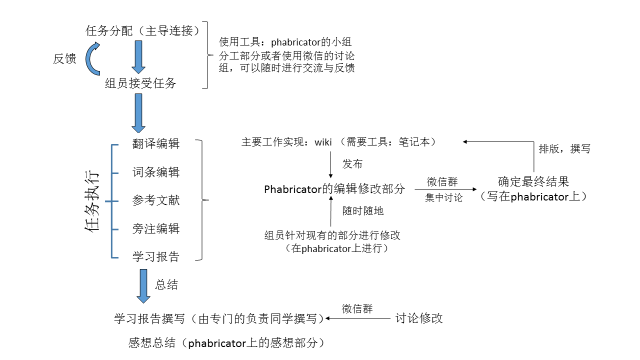
\includegraphics[width=15cm]{2.png}
   	\caption{第一组翻译时使用的结构}
   \end{figure}
   
   在现代社会随着科技的不断发展,知识的复杂度也在不断的加剧,人类的认知方式也在不断的发生改变,因此如何构建一个良好的认知结构框架是一个非常重要的问题,而科技的不断发展给我们提供了这样一个机会,过去人类的认知只能通过书籍,或者面对面的交流,但随着互联网的不断发展以及科技的不断进步,越来越多的开源软件,例如:Wiki , Phabricator , Github 等,和很多智能工具的出现,例如:智能手机,笔记本电脑,Google glasses,等,我们完全可以实现一个随时随地学习的结构框架,这样能够让我们无论处在怎样的环境下都能够保持认知的状态。

   我们小组在这本书的翻译工作上就设想了这样一种结构,示意图如图3.1所示:

   可见我们组通过使用不同的工具,实现的随时随地的进行翻译工作以及相互交流学习讨论,使得我们能够高效率的进行学习,并且能够及时的进行反馈。
\section{第二组:大有若无}

大有若无是我们的实现思路、想法,以通用的技术支持,不给使用者施加任何限制,达到能让使用者随时随地使用数字出版物、学习的目的,最终达到开花结果的效果。

Modelica其实就是类似“大有若无”的思路,他应用函数仿制的方法,以达到节约资源的目的。有一种通用的硬件和函数,但不给用户施加限制,通过函数仿制达到让用户建立各种模型和仿真的目的。或者说我们“大有若无”的思路就是类似于Modelica。

大有若无是我们组的主题,大有若无这一词看起来有些荒谬,但其实代表的是为使用者提供的自由。佛学中常常提到大有若无一词,有否极泰来之意。我们组希望我们所制作的数字化出版物或者其他的平台构想能够给使用者足够的自由度。

对于大有若无,我们可以从以下两个方面来看。

首先从我们的思想上,我们在翻译工作和团队协作甚至是自己的学习报告中多可以体现这种大有若无的思想,那么这种思想的体现,其实就是自由,即之前我们小组的同学提到的,我们思考问题是不能有过多的局限和约束,这样会使我们的产品和成果创新性和质量大大降低,所以我们我们的翻译工作及数字出版物中不能缺少这种思想,我们虽然是在按照英文书籍翻译,但翻译的自由度确实极大,比如上节课老师提到的墨子的兼爱非攻就会在翻译中产生明显的效果,即数字出版物的灵活翻译是大有若无的体现之一。

另外,我们的数字出版物的制作完善过程伴随着多种软件的使用,比如Wiki, Git, Phabricator等的使用,这些工具大大减少了我们翻译工作的复杂程度,我们无需在看纸质的英文书籍来翻译,也无需再在纸质的翻译上做修改,当然,便捷还不止这些,我们可以随时随地的用各种设备进行浏览,查阅别人对于我们数字出版物的反馈和修改。这些翻译过程中复杂度的简化也是我们小组提出的大有若无的体现。

\section{第三组:开花结果}

我们组的主题是开花结果。一切产品和设计理念,不论使用怎样的工具和何等的手法,最终都要以产品结果的优劣来进行第一顺序的评判。不论是Wiki、GitHub亦或是Phabricator,都是我们在实现产品优质结果中选择的最优化工具。我们所做的工作,在以上几种工具尤其是wiki中,能够很好地转化为可视化的结果,并且能迅速给予相关的评判标准以帮助我们完善这一结果。

我们在践行开花结果这一理念时,主要从工作流程,工作状态,工作结果考量这几个方面进行。

首先是工作流程,为了达到较好的结果,需要小组内部成员合理地分工协作。每周在课程结束后,我们就会召开小组内部的工作讨论会,在会议上制定本周的工作计划。随后我们利用Wiki或Phabricator进行任务责任归属的认定,最终完成工作。我们在工作流程和逻辑模型中认真考虑了结果的优劣,以此制定出最优化结果的工作协议。

其次是我们的工作状态。在Wiki上,我们小组承担了四个章节的翻译、添加注释、添加词条等工作,翻译前前后后修改共计11次,累计添加词条40余条,全部达到了参考文献的标识和词条的本地化。我们所进行的所有工作都秉承着期望最优结果进行。

最后是我们的工作结果。最直接的就是Wiki上的四章翻译、注释、词条。这些结果都十分精致,达到了之前所期望的开花结果的状态。除此之外,我们还精心选择了贴合的结果呈现方式,比如wiki注释中我们选择分栏并且将分栏代码简单化;Phabricator和小组协作框架冲突时进行大量讨论,最后适应在Phabricator中的工作模式。

而在课程之外,我们更希望希望在对自己的认知有彻底的改变之后,能真正的影响到自己对自身的要求,能按照新的思维和认知生活学习,在人生中也开花结果。


%\chapter*{Bibliography}
%\addcontentsline{toc}{chapter}{\textcolor{ocre}{Bibliography}}
%\section*{Books}
%\addcontentsline{toc}{section}{Books}
%\printbibliography[heading=bibempty,type=book]
%\section*{Articles}
%\addcontentsline{toc}{section}{Articles}
%\printbibliography[heading=bibempty,type=article]

%----------------------------------------------------------------------------------------
%	INDEX
%----------------------------------------------------------------------------------------

\cleardoublepage
\phantomsection
\setlength{\columnsep}{0.75cm}
\addcontentsline{toc}{chapter}{\textcolor{ocre}{Index}}
\printindex

%----------------------------------------------------------------------------------------

\end{document}
